\documentclass[9pt]{beamer}
\usepackage{beamerpreamble}
\usepackage[swedish]{babel}
\usepackage{minted}
\usepackage{comment}
\usemintedstyle{vs}
\usepackage{xcolor}
\usepackage{tikz}
\usepackage{textgreek}
\usepackage{dirtytalk}

\renewcommand{\ttdefault}{cmtt}

\newcommand*\mean[1]{\bar{#1}}

\title{Datalaboration - Förberedande tutorial}
\author[benjamin.eriksson@physics.uu.se]{Benjamin Eriksson  \\ \tiny{med inspiration från} \\ \scriptsize{Slides av M. Isacson, M. Ellert, M. Olvegård, och B. Lindgren}}
\institute[Uppsala universitet]{{\small Avdelningen för tillämpad kärnfysik \\ Institutionen för fysik och astronomi} \\ \uulogo}
\date{{\small Reviderad}\\ \today}

\begin{document}

    \begin{frame}{Osäkerhetspropagering}
        Efter denna föreläsning ska du kunna
        \begin{itemize}
            \item beskriva vad som menas med osäkerhetspropagering
            \item beräkna osäkerheten för en funktion som beror på flera variabler med olika osäkerheter
        \end{itemize}
    \end{frame}

    \begin{frame}{Osäkerhetspropagering}
        Vi är intresserade av en storhet $y$ som är en funktion flera oberoende mätningar $x_i$,
        \begin{equation*}
            y = f(x_1, x_2, \ldots, x_n)
        \end{equation*}
        där vi har osäkerheter i varje mätning $u_{x_1}$, $u_{x_2}$, ..., $u_{x_n}$.
        
        \vspace{0.2cm}
        Mätosäkerheten i $y$ beror då på mätosäkerheterna i $x_i$,
        \begin{equation*}
            u_y = \sqrt{\sum_{i=1}^n\left(u_{x_i}\frac{\partial f}{\partial x_i}\right)^2}
        \end{equation*}

        \begin{columns}[T]
            \column{.5\textwidth}
                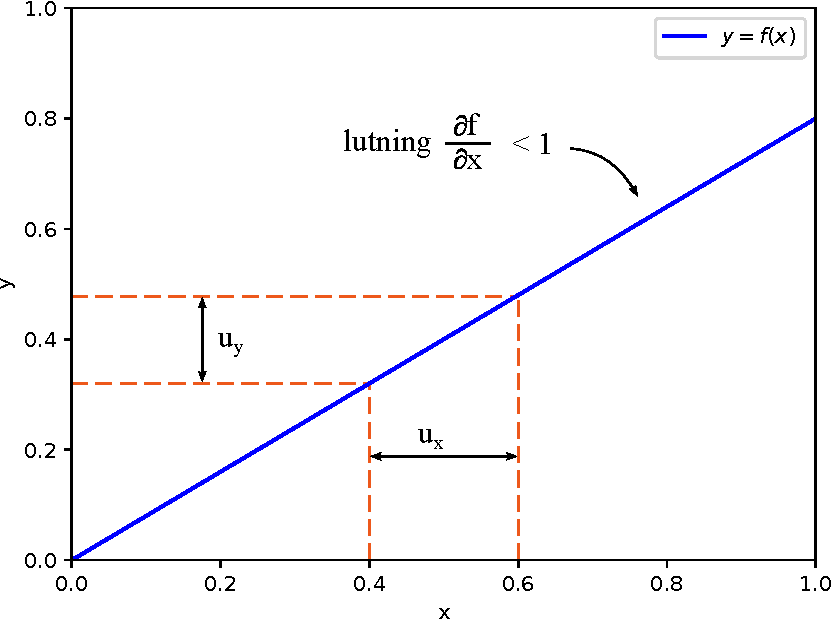
\includegraphics[width=\textwidth]{Fig_1_new.pdf}\\
            \column{.5\textwidth}
                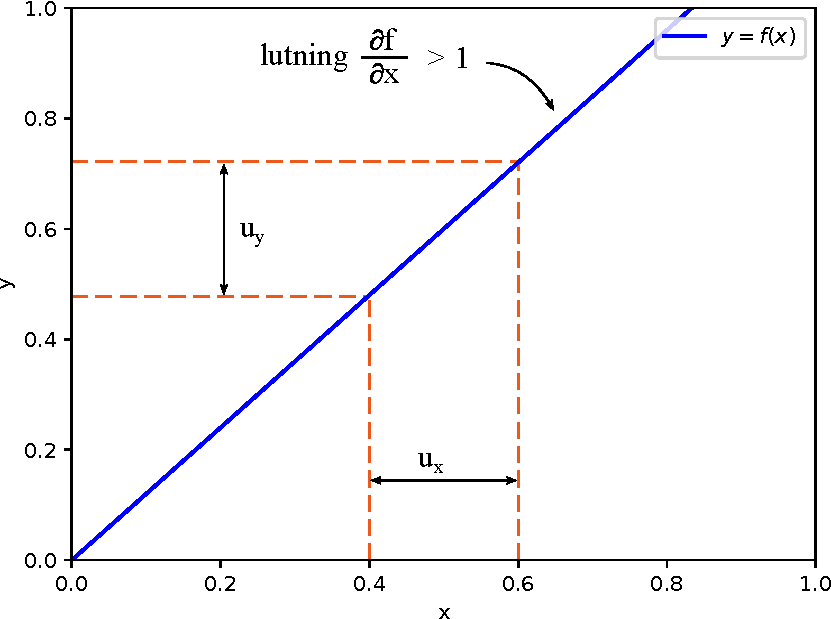
\includegraphics[width=\textwidth]{Fig_2_new.pdf}\\
        \end{columns}
    \end{frame}


    \begin{frame}
        \hrule
        \vspace{0.1cm}
        \textcolor{red}{Exempel}: 
        Volymen $V$ av en cylinder beror på radien $r$ och höjden $h$
        \begin{equation*}
            V(r, h) = \pi r^2 h
        \end{equation*}
        Vi mäter $r$ och $h$ och uppskattar mätosäkerheterna till $u_r$ och $u_h$. Vad är osäkerheten $u_V$ i volymen $V$?
        \vspace{0.1cm}
        \hrule
        \vspace{0.2cm}
        Vi har formeln för osäkerhetspropagering
        \begin{equation*}
            u_y = \sqrt{\sum_{i=1}^n\left(u_{x_i}\frac{\partial f}{\partial x_i}\right)^2}
        \end{equation*}
        
        vilket med vår funktion för volymen blir
        \begin{equation*}
            u_V = \sqrt{\left(u_r\frac{\partial V}{\partial r}\right)^2 + \left(u_h\frac{\partial V}{\partial h}\right)^2}
        \end{equation*}
        \pause
        med partiella derivator
        \begin{equation*}
            \frac{\partial V}{\partial r} = 2\pi r h, \quad \frac{\partial V}{\partial h} = \pi r^2
        \end{equation*}

    \end{frame}
    
    \begin{frame}
        \hrule
        \vspace{0.1cm}
        \textcolor{red}{Exempel}: 
        Volymen $V$ av en cylinder beror på radien $r$ och höjden $h$
        \begin{equation*}
            V(r, h) = \pi r^2 h
        \end{equation*}
        Vi mäter $r$ och $h$ och uppskattar mätosäkerheterna till $u_r$ och $u_h$. Vad är osäkerheten $u_V$ i volymen $V$?
        \vspace{0.1cm}
        \hrule
        \vspace{0.2cm}
        Detta ger att
        \begin{align*}
            u_V &= \sqrt{\left(u_r\frac{\partial V}{\partial r}\right)^2 + \left(u_h\frac{\partial V}{\partial h}\right)^2} =
            \sqrt{(u_r 2\pi r h)^2 + (u_h \pi r^2)^2} \\
            &= \pi r^2 h \sqrt{4\left(\frac{u_r}{r}\right)^2 + \left(\frac{u_h}{h}\right)^2}
            = V \sqrt{4\left(\frac{u_r}{r}\right)^2 + \left(\frac{u_h}{h}\right)^2}
        \end{align*}
        d.v.s. mätosäkerheten i $V$ är
        \begin{align*}
            u_V = V\sqrt{4\left(\frac{u_r}{r}\right)^2 + \left(\frac{u_h}{h}\right)^2}
        \end{align*}
    \end{frame}
    
\end{document}